\documentclass[english,twoside, openright, hidelinks, 11 pt, class=report,crop=false]{standalone}
\input{../../preamb}



\begin{document}
{\Large Eksamen 1T våren 2025\hfill \\ {\footnotesize Løsning fra \color{blue} \href{https://sindreheggen.wordpress.com/}{OpenMathBooks prosjektet}}}	

\subsection*{Oppgave 1}
Nevneren til $f$ er lik 0 bare hvis $x=-\frac{1}{2}$. For denne $x$-verdien er telleren til $f$ lik $-9$, og dermed har vi at $\lim\limits_{x\to-\frac{1}{2}}f=\pm\infty$. Altså er $x=-\frac{1}{2}$ den vertikale asymptoten til $f$. \vsk

Vi kan skrive $f$ som
\[ f=\frac{12x-3}{2x+1}=\frac{12x-3+6-6}{2x+1}=\frac{12x+6}{2x+1}-\frac{9}{2x+1}=6-\frac{9}{2x+1} \]
Dette betyr at $\lim\limits_{x\to|\infty|}f=6$. Dermed er $y=6$ den horisontale asymptoten til $f$.

\subsection*{Oppgave 2}
Da $2(-6)=-12$ og $2+(-6)=-4$, er
\[ x^2-4x-12=(x+2)(x-6) \]
\textbf{Alternativ 1}\\
Vi lager et fortegnsskjema:
\begin{figure}
	\centering
	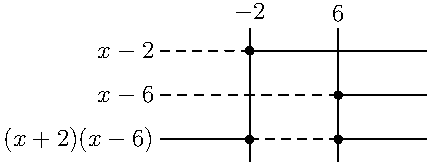
\includegraphics{opg1del1}
\end{figure}
Altså er $x\in(-2, 6)$. \vsk

\textbf{Alternativ 2}\\
Da uttrykket er et andregradsuttrykk med positivt andregradsledd, vet vi at uttrykket er konvekst. Da vet vi at uttrykket er negativt mellom 0-punktene. Altså er $x\in(-2, 6)$.

\subsection*{Oppgave 3}
Gitt
\[ f(x)=ax^2+bx+c \]
Hvis $f$ bare har ett nullpunkt, har vi av \textit{abc}-formelen at
\[ b^2-4ac=0 \]
Videre har vi at
\[ f(0)=c=9 \]
Altså er
\[ b^2-36a=0 \]
Setter vi $a=1$, kan $b$ være lik 6. Da er
\[ f(x)=x^2+6+9 \]
\newpage
\subsection*{Oppgave 4}
\abc{
\item Vi ser at $x=1$ er en løsning av ligningen. Vi polynomdividerer uttrykket med $x-1$:
\alg{
	\phantom{-}&(x^3-7x^2-10x+16):(x-1) = x^2-6x-16\\ 
	-&\underline{(x^3-x^2)} \\
	&\phantom{\,x\;}-6x^2-10x+16  \\
	&\phantom{}-\underline{(-6x^2+6x)}\\
	&\phantom{aaaaa\;''}-16x+16 \\
	&\phantom{aaaa\,}-\underline{(-16x+16)} \\
	&\phantom{aaaaaaaaaaaaaaa}0
}
Da $2(-8)=-16$ og $2+(-8)=6$, er
\[ x^2-6x-16=(x+2)(x-8) \]
Altså er
\[ x^3-7x^2-10x+16=(x-1)(x+2)(x-8) \]
Uttrykket over er lik 0 for $x\in{-2, 1, 8}$.
\item Av oppgave a) vet vi at $f$ har to nullpunkt langs den positive siden av $x$-aksen. Og da tredjegradsutrtrykket er positivt, må $f$ være voksende for store $x$-verdieer. Det må bety at figur C kan være grafen til $f$.
}
\newpage
\subsection*{Oppgave 5}
\abc{
\item Da $\triangle ABC$ er likeseidet er $\angle A=\angle ACB=\angle B=60^\circ $. Da er $ \angle ACD=30^\circ$, og i tillegg er $AD=1$. Dermed har vi at
\alg{
\sin 30^\circ = \sin \angle A=\frac{AD}{AC}=\frac{1}{2} \vn
\cos 60^\circ = \cos \angle A=\frac{AD}{AC}=\frac{1}{2}
}
\begin{figure}
	\centering
	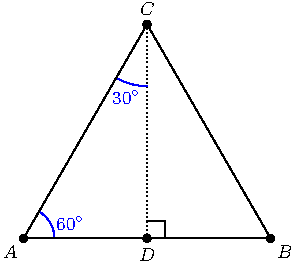
\includegraphics{opg5del1}
\end{figure}
\item Av arealsetningen, og da $\sin \angle A=\frac{1}{2}$, har vi at
\[ \text{arealet til trekanten}=\frac{1}{2}AB\cdot AC\cdot \sin \angle A=\frac{1}{2}\cdot10\cdot6\cdot\frac{1}{2}=15 \]
\item Av cosinussetningen, og da $\cos \angle P=\frac{1}{2}$, har vi at
\alg{
QR^2 &= PQ^2+PR^2-2PQ\cdot PR-2\cos \angle P \\
&= 64+9-8\cdot3 \\
&= 49
}
Da $QR>0$, er $QR=\sqrt{49}=7$
}

\subsection*{Oppgave 6}
Resultatet i CAS viser at ligningen er sann for alle verdier av $x$, noe som gjør ligningen til en identitet. En identitet er en ligning som er sann uansett hvilke verdier som gis til variablene som inngår i uttrykket.

\subsection*{Oppgave 7}
Progrmammet gir den minste verdien til $f(x)=x^2+2x-15$ for heltalls $x$ på intervallet $[-5, 5]$. Da $5(-3)=-15$ og $5+(-3)=2$, er
\[ f(x)=(x+5)(x-3)\]
Dermed har $f$ ekstremalpunkt på midtpunktet mellom $x=-5$ og $x=3$, som er $x=-1$. 
Da andregradsleddet til $f$ er positivt, er $f$ en konveks funksjon, og da er $x=-1$ minimumspunktet til $f$. Altså vil printet verdi være 
\[ f(-1)=-16 \]

\newpage
\subsection*{Oppgave 1}
\abc{
\item Vi skriver tallene inn i GeoGebra, og bruker \texttt{RegEks} for regresjon ved en eksponentialfunksjon (linje 8).
\item Stigningstallet til linja gjennom $(4, K(4))$ og $(21, K(21))$ er $70.24$ (linje 9). Dette betyr at mellom april i 2024 og september 2025 var den gjennomsnittlige økningen i antall tilfeller lik $70.24$ tilfeller per måned.
\item I mai 2025 vil det bli registrert 5336 tilfeller i følge modellen (linje 10).
}

\begin{figure}
	
\includegraphics[scale=0.3]{opg1}
\end{figure}
\newpage
\subsection*{Oppgave 2}
Vi setter antall liten sekk lik $x$ og antall stor sekk lik $y$, og løser ligningssettet i CAS. Får da at det ble solgt 32 små sekker og 48 store sekker.
\begin{figure}
	\centering
	
\includegraphics[scale=0.4]{opg2}
\end{figure}

\subsection*{Oppgave 3}
\abc{
\item Arealet til én av de 12 trekantene er gitt i linje 1. Totalt areal lik 120 gir ligningen i linje 2. Dermed er diameteren lik $4\sqrt{10}$.
\item Vi setter den ukjente siden i trekantene lik $x$. Da trekantene er likebeinte, er $x$ gitt av ligningen i linje 4. Omkretsen er dermed gitt i linje 6.
}
\begin{figure}
	\centering
	
\includegraphics[scale=0.45]{opg3}
\end{figure}
\newpage
\subsection*{Oppgave 4}
\abc{
	\item \texttt{definer funksjon antall\_kvadrat(n) = n**2+2*n+1} \\
	
	\texttt{for n<21: print antall kvadrat}\os
	Funksjonen for antall kvadrater kommer av at det er $n^2$ kvadrat som utgjør et større kvadrat, $n$ kvadrat utgjør et større rektangel, og $n+1$ kvadrat ligger på skrå.
	\item \phantom{} \python{opg4b.py}
	\item \phantom{} \python{opg4c.py}
	Får at det blir igjen 15017 kvadrat når 142 figurer er lagd.
}
\newpage
\subsection*{Oppgave 5}
\abc{
\item Bruker Excel til å fylle ut tabellen.
\begin{figure}
	\centering
	
\includegraphics[scale=0.5]{opg5a}\\[12pt]
	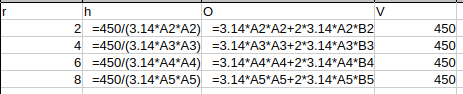
\includegraphics[scale=0.5]{opg5a2}
\end{figure}
\item Vi har at
\[ h=\frac{450}{\pi r^2} \]
Dermed er
\[ O=\pi r^2+2\pi r \cdot \frac{450}{\pi r^2} =\pi r^2+\frac{900}{r}  \]
Vi skriver dette utrykket for $O$ inn i GeoGebra (linje 1).
\item Vi ser at $O$ har et bunnpunkt mellom $r=2$ og $r=8$, og bruker GeoGebra-kommandoen \texttt{Ekstremalpunkt} til å finne at i bunnpunktet er $r\approx5.2$ og $O\approx258$ (linje 2). (Ut ifra funksjonsuttrykket er det åpenbart at dette er det eneste bunnpunktet for $r>0$) 
\begin{figure}
	\centering
	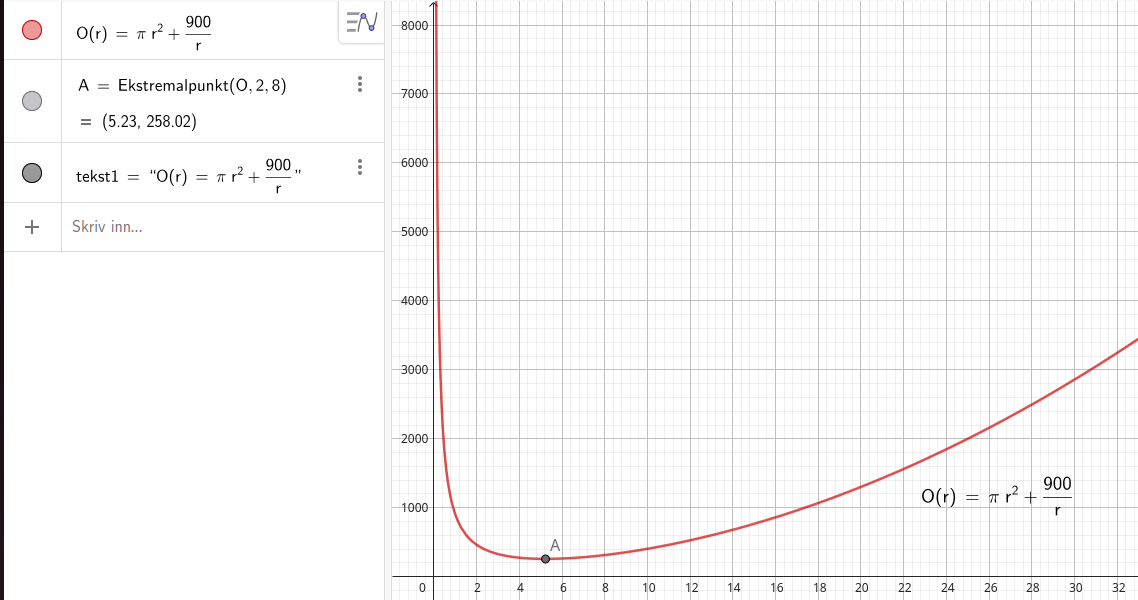
\includegraphics[scale=0.2]{opg5bc}
\end{figure}
}

\subsection*{Oppgave 6}
For $f$ har vi at
\begin{itemize}
\item De vertikale asymptotene ser ut til å ha lik avstand til $y$-aksen. Velger derfor to faktorer i nevner som går mot 0 når $x=2$ eller $x=-2$.
\item Nullpunktet til $f$ er på positiv side av $x$-aksen og til venstre for den positive vertikale asymptoten. Prøver derfor med $x-1$ i teller, som gir rett form på grafen og skjæring med $y$-aksen på positiv side.
\item Bruker GeoGebra-kommandoen \texttt{Asymptote} for å bekrefte at asymptotene er riktige (linje 3).
\end{itemize}
For $g$ har vi at
\begin{itemize}
	\item Funksjonen har ingen vertikal asymptote. Prøver derfor med $x^2+1$ i nevner for å sikre nevner forkskjellig fra 0.
	\item Funksjonen har et nullpunkt på negativ side av $x$-aksen. Prøver derfor med $x+1$ i teller, som gir rett form på grafen og skjæring med $y$-aksen på positiv side.
	\item Bruker \texttt{Asymptote} for å bekrefte at asymptotene er riktige (linje 4).
\end{itemize}
\begin{figure}
	\centering
	
\includegraphics[scale=0.4]{opg6}
\end{figure}
\end{document} 